%%%%%%%%%%%%%%%%%%%%%%%%%%%%%%%%%%%%%%%%%%%%%%%%%%%%%%%%%%%%%%%%%%%%%%%%%%%%%%%%
%2345678901234567890123456789012345678901234567890123456789012345678901234567890
%        1         2         3         4         5         6         7         8

\documentclass[letterpaper, 10 pt, conference]{ieeeconf}  % Comment this line out
                                                          % if you need a4paper
%\documentclass[a4paper, 10pt, conference]{ieeeconf}      % Use this line for a4
                                                          % paper

\IEEEoverridecommandlockouts                              % This command is only
                                                          % needed if you want to
                                                          % use the \thanks command
\overrideIEEEmargins
% See the \addtolength command later in the file to balance the column lengths
% on the last page of the document
\hbadness=15000%
\setlength{\parindent}{1cm}

% The following packages can be found on http:\\www.ctan.org
\usepackage{graphicx} % for pdf, bitmapped graphics files
%\usepackage{epsfig} % for postscript graphics files
%\usepackage{mathptmx} % assumes new font selection scheme installed
%\usepackage{times} % assumes new font selection scheme installed
%\usepackage{amsmath} % assumes amsmath package installed
%\usepackage{amssymb}  % assumes amsmath package installed

\title{\LARGE \bf
An\'alisis de Algoritmos: Similitud de Imagenes
}

%\author{ \parbox{3 in}{\centering Huibert Kwakernaak*
%         \thanks{*Use the $\backslash$thanks command to put information here}\\
%         Faculty of Electrical Engineering, Mathematics and Computer Science\\
%         University of Twente\\
%         7500 AE Enschede, The Netherlands\\
%         {\tt\small h.kwakernaak@autsubmit.com}}
%         \hspace*{ 0.5 in}
%         \parbox{3 in}{ \centering Pradeep Misra**
%         \thanks{**The footnote marks may be inserted manually}\\
%        Department of Electrical Engineering \\
%         Wright State University\\
%         Dayton, OH 45435, USA\\
%         {\tt\small pmisra@cs.wright.edu}}
%}

\author{Nicol\'as Feoli$^{1}$ y Sebastian Salas$^{2}$% <-this % stops a space
\thanks{*Estudiantes del Instituto Tecnológico de Costa Rica}% <-this % stops a space
}


\begin{document}



\maketitle
\thispagestyle{empty}
\pagestyle{empty}

%%%%%%%%%%%%%%%%%%%%%%%%%%%%%%%%%%%%%%%%%%%%%%%%%%%%%%%%%%%%%%%%%%%%%%%%%%%%%%%%
\begin{abstract}

Este art\'iculo se describe la implementaci\'on de un algoritmo gen\'etico de creaci\'on de im\'agenes en el lenguaje de programaci\'on Python versi\'on 2.7. Se utilizaron tres algoritmos de similitud de im\'agenes los cuales son descritos y analizados. Se incluye en el documento el resultado y el an\'alisis de 12 experimentos con distintas im\'agenes tanto a color como en escala de grises y su efectividad con los distintos algoritmos implementados.
\end{abstract}


%%%%%%%%%%%%%%%%%%%%%%%%%%%%%%%%%%%%%%%%%%%%%%%%%%%%%%%%%%%%%%%%%%%%%%%%%%%%%%%%
\section{\textbf{INTRODUCCI\'ON}}

Desde la creaci\'on de las im\'agenes digitales hasta la actualidad, se ha venido revolucionando su calidad y usos. Estas est\'an presentes en la vida cotidiana de las personas. Una imagen o desde un punto de vista m\'as computacional un arreglo bidimensional de pixeles pueden ser generadas desde im\'agenes aleatorias mediante algoritmos gen\'eticos.\\
\indent Estos algoritmos, implementados especialmente en la inteligencia artificial, son inspirados en la evoluci\'on biol\'ogica y su base gen\'etico-molecular. Estos  funcionan entre el conjunto de soluciones de un problema llamado fenotipo, y el conjunto de individuos de una poblaci\'on natural, codificando la informaci\'on de cada soluci\'on en una cadena, generalmente binaria, llamada cromosoma. Los s\'imbolos que forman la cadena son llamados los genes. Cuando la representaci\'on de los cromosomas se hace con cadenas de d\'igitos binarios se le conoce como genotipo. \\ 
\indent Los cromosomas evolucionan a trav\'es de iteraciones, llamadas generaciones. En cada generaci\'on, los cromosomas son evaluados usando alguna medida de aptitud. Las siguientes generaciones (nuevos cromosomas), son generadas aplicando los operadores gen\'eticos repetidamente, siendo estos los operadores de selecci\'on, cruzamiento, mutaci\'on y reemplazo.\\ 
\indent Dentro de las funciones de adaptabilidad se utilizaron los siguientes algoritmos: distancia euclideana, mean square error y la creaci\'on de uno propio. En cuanto a la distancia euclideana se usa para comparar dos vectores que en este caso ser\'an de pixeles y el error cuadr\'atico medio mide el promedio de los errores al cuadrado, es decir, la diferencia entre el estimador y lo que se estima. El algoritmo propio se basa en que si el pixel x es diferente al mismo pixel de la imagen meta, a ese se le suma uno para generar una nueva poblaci\'on. 

\section{\textbf{Complejidad Algor\'itmica}}

\subsection{\textbf{An\'alisis Formal del Algoritmo Propio}}

\setlength{\parindent}{1cm}Se asignar\'a una unidad de tiempo a las declaraciones, asignaciones, operaciones simples $(+, -, *, /)$. A continuaci\'on, el fragmento de c\'odigo del algoritmo.\\ 

def calcularAdaptabilidad (individual):\\ 
\indent\indent fitness = 0\\ 
\indent\indent for i in range(len(individual)):\\ 
\indent\indent\indent if individual[i] == listaGenesMeta[i]: \\ 
\indent\indent\indent\indent fitness += 1\\ 
\indent\indent return fitness \\ 

\indent Observe que primero se tiene una inicializaci\'on, lo que nos da 1 unidad de tiempo. Luego se tiene un ciclo for que ejecuta un aumento $n + 1$ veces (n por la cantidad de elementos que tenga la lista de pixeles de la imagen (tama\~no) lo cual equivale a $(n+1)$ unidades.\\ 
\indent Dentro del for se tienen 2 unidades de tiempo aproximadamente por la comparaci\'on que se tiene y el retorno interno del for. Esto se realiza n veces, por lo que la complejidad de esta secci\'on será $2*n$.\\ 
\indent En el mismo for tenemos una estructura if que tiene un incremento que cuenta por una unidad de tiempo 1n. Por \'ultimo, un retorno, al cual se le puede asignar una unidad de tiempo.\\ 
\indent Si unimos los datos nos queda una complejidad total aproximada del algoritmo de: \\ 

\indent\indent $1+(n+1)+2n+ 1n+1$\\ 
\indent\indent $=n+1+3n +2$\\ 
\indent\indent $=4n+3$

\begin{figure}[h]
\centering
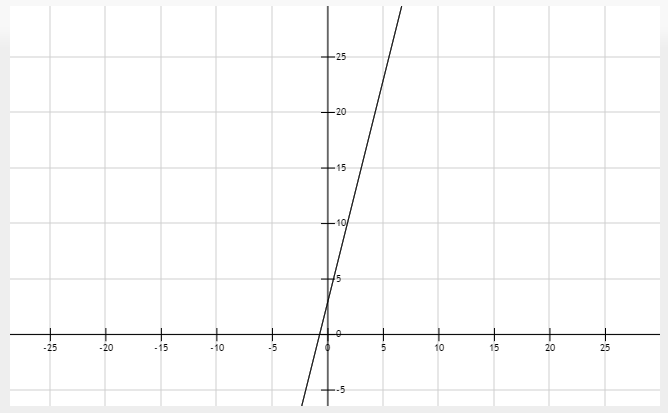
\includegraphics[width=5cm, height=5cm]{GraficaPropia}
\end{figure}


\indent \textbf{Nota:} Otra manera de visualizarlo ser\'ia  $Cn + C$ donde $C$ equivale a una constante de tiempo que requiere el proceso. \\ 
\indent Dado que se desea obtener la complejidad, se pueden eliminar los valores que no crecer\'an más que $n$ y la constante que la multiplica. Lo que nos da $O(n)$.


\subsection{\textbf{An\'alisis Formal del Algoritmo MSE}}

\indent De igual manera se asignar\'a una unidad de tiempo a las declaraciones, asignaciones, operaciones simples. A continuaci\'on, el fragmento de c\'odigo del algoritmo error cuadr\'atico medio.\\
def mse(imageA):\\
\indent for i in range(len(imagenA)):\\
\indent \indent errorCM += (np.array(imageA) - np.array (listaGenesMeta)) ** 2)\\
\indent errorCM /= float(tamanoPoblacion)\\
\indent return errorCM\\

\indent El algoritmo inicia con un ciclo for que ejecuta un aumento $n + 1$ veces ($n$ por la cantidad de elementos que tenga la lista de pixeles de la imagen (tama\~no) lo cual equivale a $n+1$ unidades de tiempo. Dentro de esta estructura, hay una asignaci\'on, dos conversiones de lista, una resta y elevado potencial lo cual cuentan como $5$ unidades de tiempo extra por el total de ciclos $n$.\\
\indent Al final del algoritmo se tiene una asignaci\'on, operaci\'on simple y una conversi\'on de tipo, lo que nos da $3$ unidades de tiempo y adem\'as, un retorno, al cual de igual manera cuenta como una una unidad de tiempo m\'as $(+4)$.\\
\indent Si unimos los datos nos queda una complejidad total aproximada del algoritmo de: \\\\
\indent\indent (n+1)+5n+4=\\
\indent\indent n+1+5n +4=\\
\indent\indent 6n+5\\\\
\begin{figure}[h]
\centering
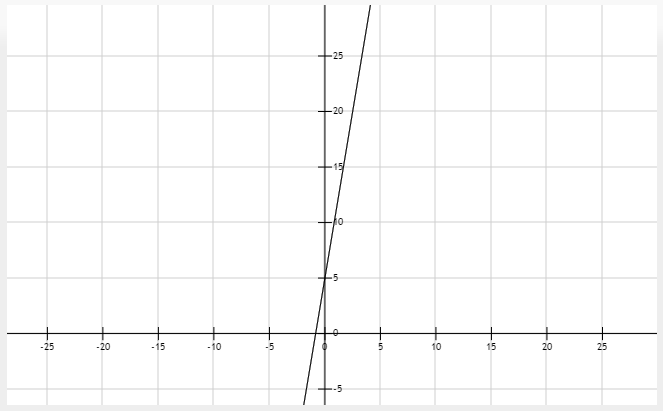
\includegraphics[width=5cm, height=5cm]{GraficaMSE}
\end{figure}
\indent Dado que se desea obtener la complejidad, como vimos en el ejemplo anterior podemos eliminar los valores que no crecer\'an m\'as que $n$ y la constante que la multiplica. Lo que nos da $O(n)$.

\section{\textbf{Metodología}}

\setlength{\parindent}{1cm}La investigaci\'on cont\'o una serie de pruebas que nos permitieran comparar los tres diferentes algoritmos de adaptabilidad que buscar\'an la similitud entre dos im\'agenes.

\begin{tabbing}
\textbf{Prueba} \=	\textbf{Algoritmo} \=	\textbf{Color}	 \=\textbf{Dimensiones}	 \=\textbf{Generation}	 \=\textbf{Imagen}\\
Casa 1 \>	MSE\>	L	\>32 X 32	\>20.000	\>Luigi.jpg\\
Caso 2 \>	MSE\>	RGB	\>32 X 32\>	20.000	\>Luigi.jpg\\
Caso 2.2\>	MSE	\>RGB	\>32 X 32\>	10.000	\>Luigi.jpg\\
Caso 3	\>MSE	\>RGB	\>50 X 50	\>20.000	\>Zelda.jpg\\
Caso 3.1\>	MSE\>	L	\>50 X 50\>	10.000	\>Zelda.jpg\\
Caso 4	\>Euclideana\>	L\>	32 X 32\>	20.000\>	Zelda.jpg\\
Caso 5	\>Euclideana\>	L\>32 X 32	\>10.000	\>Estrella.jpg\\
Caso 5.1\>	Euclideana\>	RGB	\>32 X 32\>	20.000	\>Estrella.jpg\\
Caso 6	\>Propia\>	RGB\>	32 X 32	\>20.000	\>Estrella.jpg\\
Caso 7	\>Propia\>	RGB\>	32 X 32\>	20.000	\>Print.jpg\\
Caso 8	\>Propia\>	L\>	32 X 32\>	20.000\>	Print.jpg\\
Caso 8.1 \>	Propia	\>L\>	32 X 32\>	10.000\>	Print.jpg\\
\end{tabbing}

\indent La captura de datos se realiz\'o positivamente; para efectos demostrativos mostraremos tres casos bajo las mismas condiciones para poderlas compararlas. A continuaci\'on, se mostrar\'an tres resultados donde vendr\'a la imagen de evoluci\'on de generaciones (se lee de arriba hacia abajo, de izquierda a derecha), la primer gr\'afica contiene el comportamiento de los pixeles de cuatro generaciones ($2000,5000,10000,20000$) y la segunda gr\'afica se compara la mejor generaci\'on (20000) contra los pixeles de la imagen meta.\\


\subsection{\textbf{Resultado - Caso 1 (MSE)}}

\begin{figure}[h]
\centering
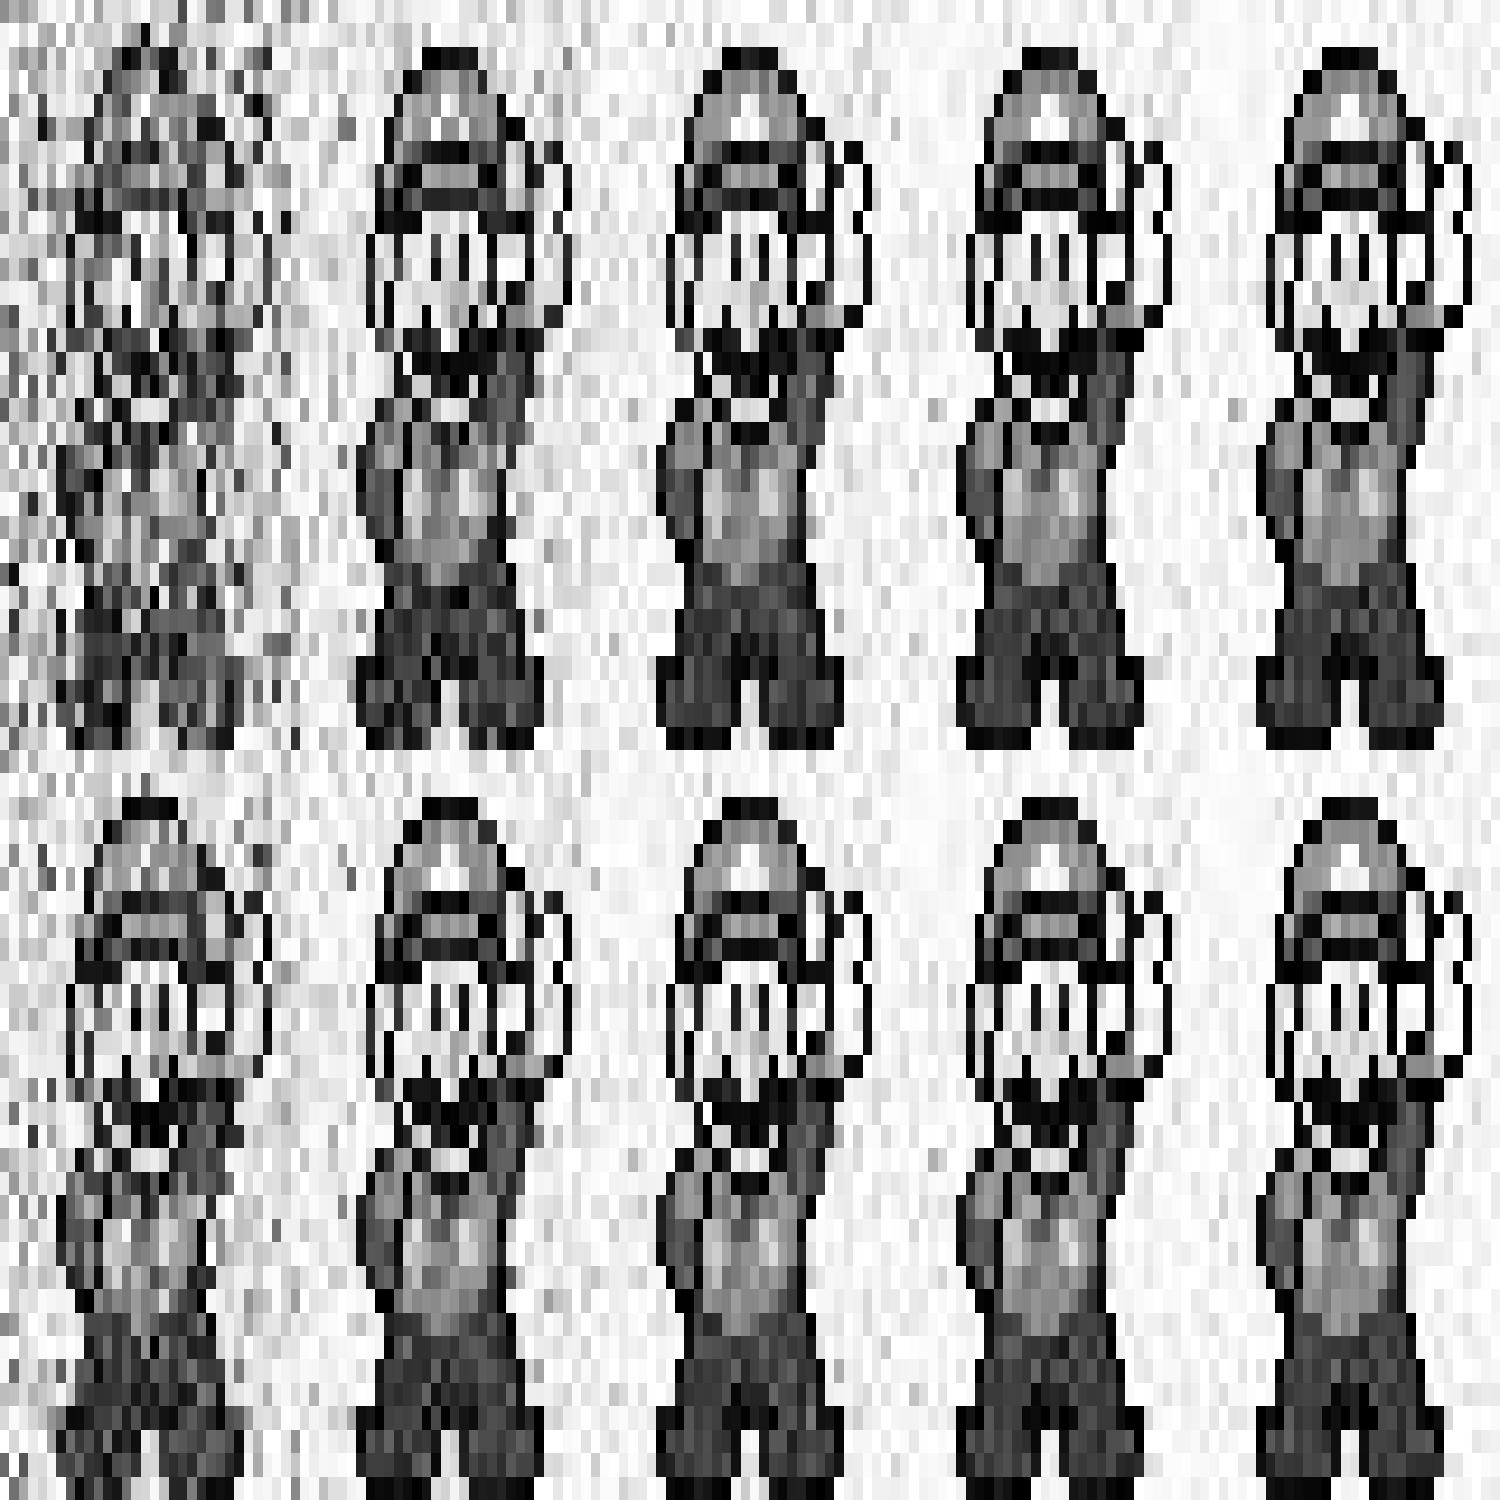
\includegraphics[width=5cm, height=5cm]{Collage}
\end{figure}
\begin{figure}[h]
\centering
\includegraphics[width=5cm, height=5cm]{MejorGeneracion1}
\end{figure}
\subsection{\textbf{Resultado - Caso 5 (Euclidiana)}}

\begin{figure}[h]
\centering
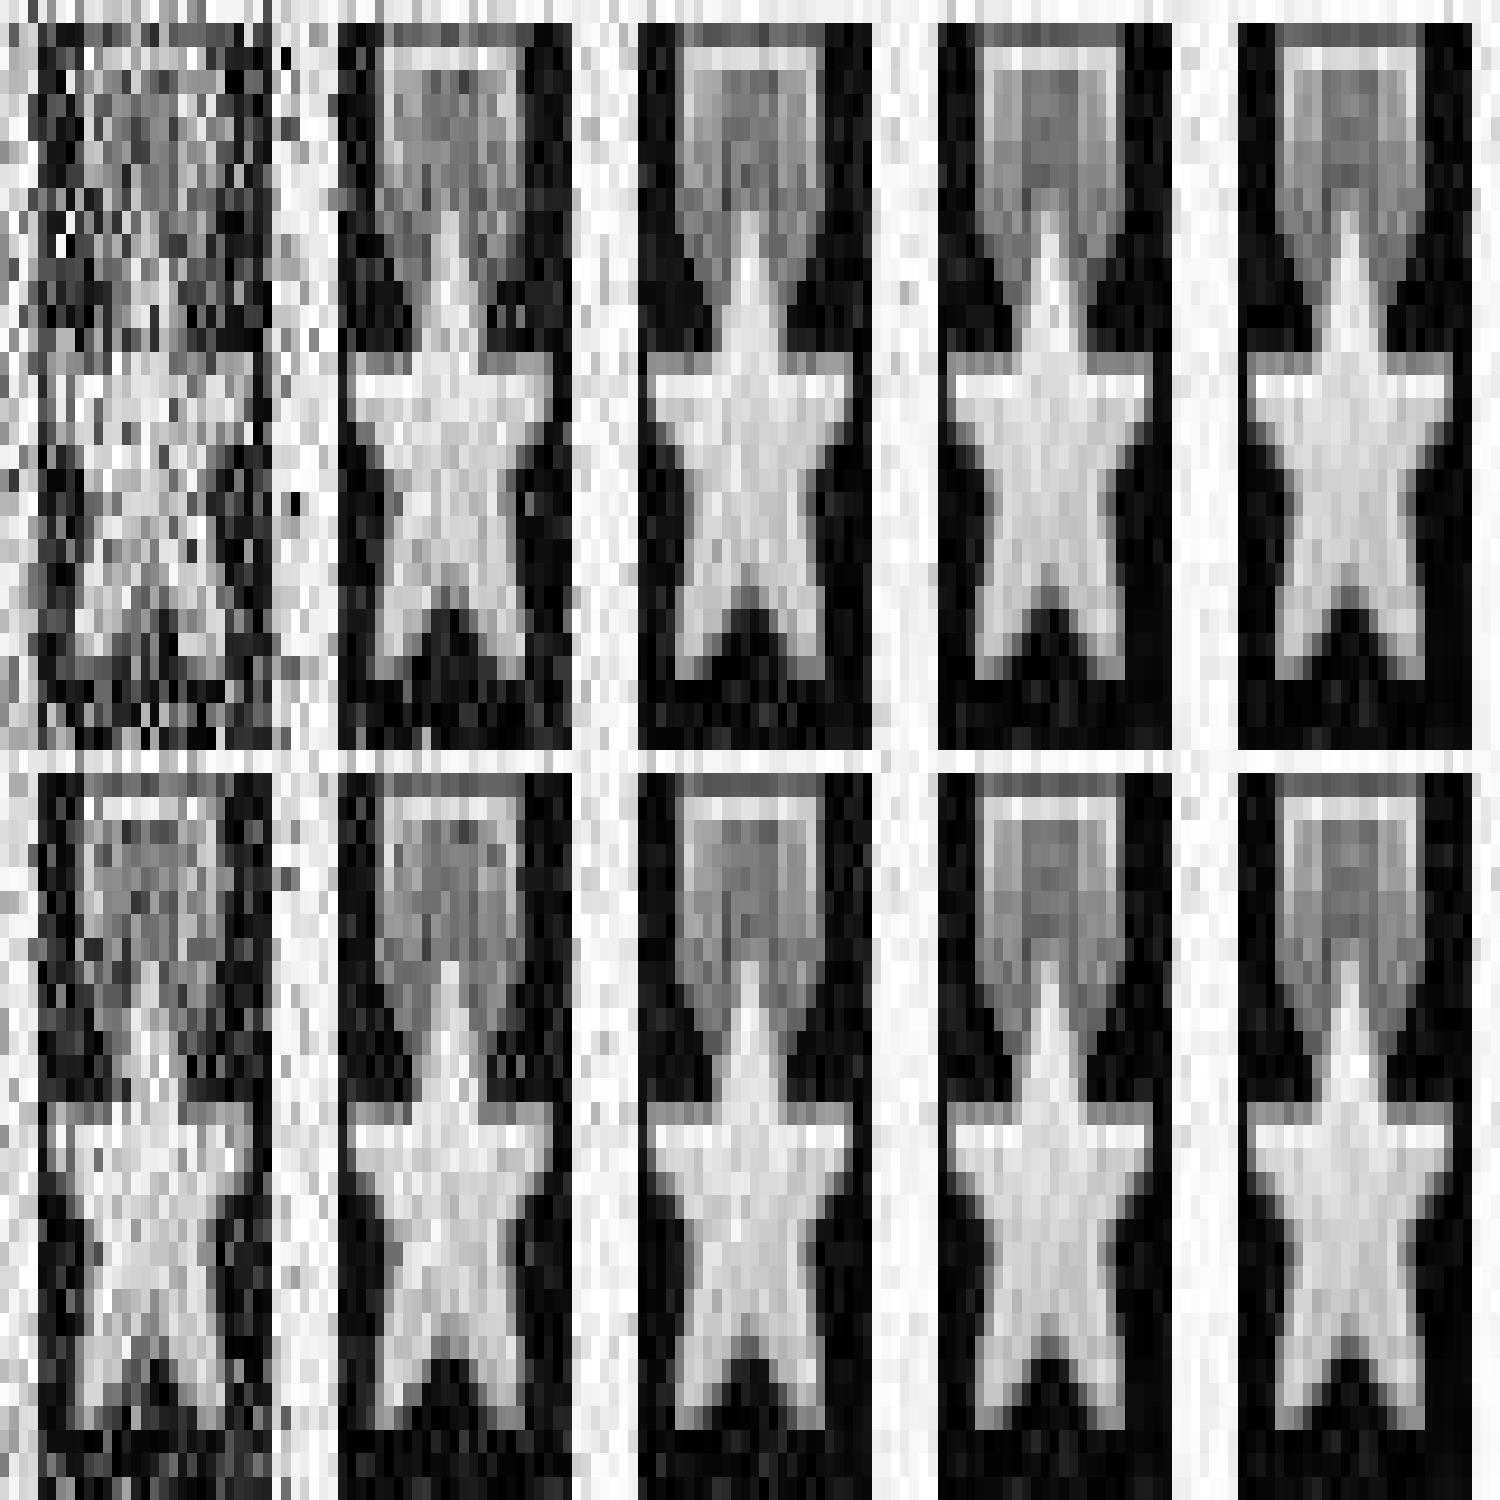
\includegraphics[width=5cm, height=5cm]{Collage1}
\end{figure}
\begin{figure}[h]
\centering
\includegraphics[width=5cm, height=5cm]{MejorGeneracion5}
\end{figure}

\subsection{\textbf{Resultado - Caso 8 (Propia)}}

\begin{figure}[h]
\centering
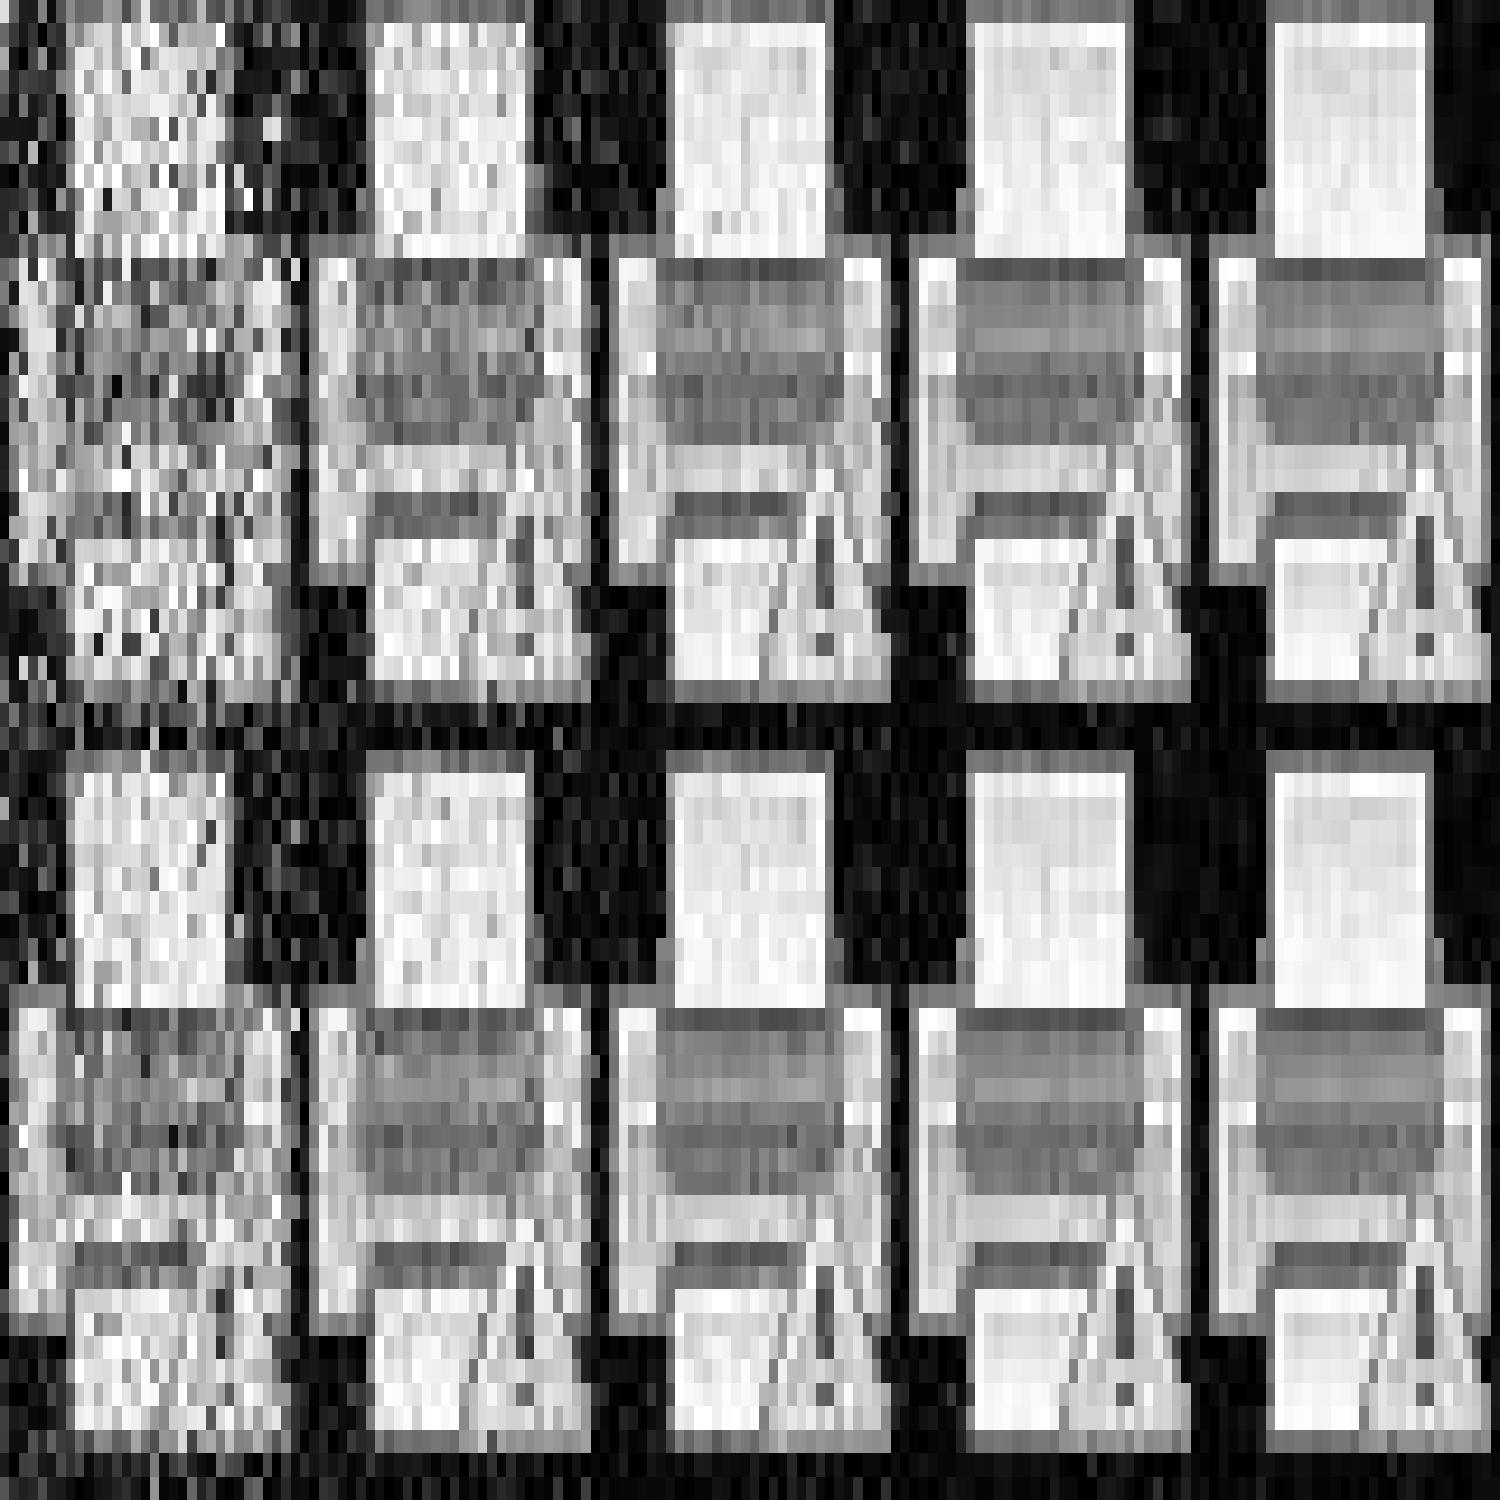
\includegraphics[width=5cm, height=5cm]{Collage2}
\end{figure}

\begin{figure}[h]
\centering
\includegraphics[width=5cm, height=5cm]{MejorGeneracion8}
\end{figure}



\section{\textbf{Discusiones}}

\setlength{\parindent}{1cm}Como se muestra en los resultados, al procesar las im\'agenes se dieron evoluciones positivas obtenido la imagen meta casi a un 90\%  aunque no se lleg\'o a converger en su totalidad. Nuestro experimento se bas\'o en manejar entre $20.000$ y $10.000$ generaciones, las cuales, las primeras a como fue de esperar, fueron bastantes malas y denotan que nuestros algoritmos ser\'ian ineficientes para pocas generaciones como por ejemplo $1000$ ya que son muchos pixeles que se deben ajustar. \\
\indent Desde el punto de vista te\'orico podemos afirmar que bajo nuestro análisis de que la euclidiana es $O(mxn)$, nuestro propio algoritmo es $O(n)$ y Mean Square Error - MSE es $O(n)$ se recomienda cualquier algoritmo para aplicar poblaciones pequenas.\\
\indent Desde el punto de vista pr\'actico si esperamos una respuesta satisfactoria no es recomendable usar estos algoritmos para im\'agenes de m\'as $100 x 100$ pixeles ya que las cantidades de comparaciones que se realizan para computadores con procesadores est\'andar requieren de mucho tiempo para poder llegar a converger una imagen. Para problemas de alta complejidad las funciones de evaluaci\'on pueden tornarse demasiado costosas en t\'erminos de tiempo y recursos.\\
\indent Visualizando las gr\'aficas suministradas por el programa como se hab\'ia pensado en la hip\'otesis, conforme van pasando las generaciones, las l\'ineas de pixeles se van a cercando a la imagen meta al punto que se llegan a parecer satisfactoriamente, not\'andose que las poblaciones se fueron adaptando y los genes menos aptos se fueran descartados.\\
\indent De igual manera, ejecutamos el programa con im\'agenes a color(RGB) y el comportamiento fue bastante ineficiente durante todo el proceso, sin embargo se lleg\'o a converger lo suficiente como para asemejarse con la imagen meta validando de que nuestras funciones de adaptabilidad estaban cumpliendo con su tarea.\\

\section{\textbf{Bibliograf\'ia}}
\indent Demiriz, Ayhan. (1999). Semi-Supervised Clustering Using Genetic Algorithms. http://s3.amazonaws.com/academia.edu.documents/40354638/Semi-SupervisedClustering UsingGenetic20151124-29087-s0rvnf.pdf?AWSAccessKeyId=AKIAIWOWYYGZ2Y53UL3 AExpires=1489283802Signature=dH5rD\%2BmS\%2BoAbi66SclLa3 HrVh4c\%3Dresponse-content-disposition=inline\%3B\%20filename\%3DSemi-supervisedclusteringusinggenetic.pdf.
\indent Rivera-G.(2006). A GENETIC ALGORITHM FOR SOLVING THE EUCLIDEAN DISTANCE MATRICES COMPLETION PROBLEM. http://slapper.apam.columbia.edu/bib/papers/river\_b\_99.pdf
\indent Anónimo. (2014). How-To: Python Compare Two Images http://www.pyimagesearch.com/2014/09/15/python-compare-two-images/
\indent Zhou Wang.(2004). IEEE TRANSACTIONS ON IMAGE PROCESSING, VOL. 13, NO. Image Quality Assessment: From Error Visibility to Structural Similarity. http://www.cns.nyu.edu/pub/eero/wang03-reprint.pdf


\end{document}
